
Šiame magistro baigiamame darbe yra palyginami 4 neuroninių tinklų architektūros: daugiavaizdis neuroninis tinklas, aprašytas poskyryje Daugiavaizdis konvoliucinis neuroninis tinklas, kapsulinis neuroninis tinklas, aprašytas poskyryje Tiriamo kapsulinio neuroninio tinklo architektūra, ir 2 daugiavaizdžiai kapsuliniai neuroniniai tinklai, aprašyti poskyriuose Tiriamo daugiavaizdžio kapsulinio neuroninio tinklo architektūra su vaizdų sujungimo sluoksniu ir Tiriamo daugiavaizdžio kapsulinio neuroninio tinklo architektūra su vaizdų kapsuliniu sluoksniu. Kiekvienas tiriamas dirbtinis neuroninis tinklas yra apmokomas naudojantis visais duomenimis, aprašytais poskyryje Tyrimams naudoti duomenys. Šie duomenys apmokymo metu yra padalinami į duomenų rinkinius, kurių dydžiai yra 96. Daugiavaizdžio konvoliucinio ir kapsulinio neuroninių tinklų apmokymų antram etapui duomenų rinkiniai sudaryti iš nuotraukų grupių, kuriose yra visos konkretaus 3D objekto modelio nuotraukos. Kiekvienas dirbtinis neuroninis tinklas yra apmokomas per 10 epochų. Daugiavaizdžio konvoliucinio ir kapsulinio neuroninių tinklų abu apmokymo etapai yra apmokomi po 5 epochas. Visų šiame magistro baigiamame darbe tiriamų dirbtinių neuroninių tinklų apmokymai trunka po 6-7 valandas naudojantis Kaggle sistema.

Šiame magistro baigiamame darbe bandoma optimizuoti kapsulinių neuroninių tinklų modifikacijų konfigūracijas. Pirmiausia bandoma optimizuoti šiuos tinklus naudojantis Bajeso hiperparametrų optimizavimo algoritmu, kuris yra aprašytas darbe \cite{bayes}. Toliau bandomos kitos konfigūracijos nei konfigūracijos aprašytos darbe \cite{capsNet}. Tačiau, dėl Kaggle sistemos apribojimų, nei vienas metodas neaptiko geresnių kapsulinių neuroninių tinklų modifikacijų konfigūracijų. Taip pat bandoma 
keisti mokymosi greitį. Tačiau skirtumai tarp rezultatų yra nereikšmingi.

Po kiekvienos epochos yra renkamos tikslumo metrikos: tikslumas klasifikuojant apmokymo duomenis, ši informacija pavaizduota lentelėje \ref{tbl:train} ir grafe \ref{img:train_plot}, ir tikslumas klasifikuojant testavimo duomenis, ši informacija atvaizduota lentelėje \ref{tbl:valid} ir grafe \ref{img:val_plot}. Tikslumas yra teisingai suklasifikuotų įrašų dalis klasifikuotų duomenų aibėje. Lentelių \ref{tbl:train}, \ref{tbl:valid} stulpelio pavaidinimas ir grafų \ref{img:train_plot}, \ref{img:val_plot} kreivių pavadinimas mvcnn yra daugiavaizdžio neuroninio tinklo tikslumas, capsnet - kapsulinio neuroninio tinklo tikslumas, mv\_capsnet - daugiavaizdžio kapsulinio neuroninio tinklo su vaizdų sujungimo sluoksniu tikslumas, mv\_cap\_capsnet1 - daugiavaizdžio kapsulinio neuroninio tinklo su vaizdų kapsuliniu sluoksniu ir vienu mokymosi etapu tikslumas, mv\_cap\_capsnet2 - daugiavaizdžio kapsulinio neuroninio tinklo su vaizdų kapsuliniu sluoksniu ir dviem mokymosi etapais tikslumas. Brūkšninė vertikali linija grafuose \ref{img:train_plot} ir \ref{img:val_plot} nurodo antrojo apmokymo etapo pirmąją epochą.

\begin{table}[]
\begin{tabular}{l|l|l|l|l|l}
	epocha &     mvcnn &   capsnet & mv\_capsnet & mv\_cap\_capsnet1 & mv\_cap\_capsnet2 \\ \hline
	0 &  0.687898 &  0.119029 &   0.517437 &        0.281199 &        0.217937 \\
	1 &  0.859519 &  0.528616 &   0.793225 &        0.806504 &        0.624331 \\
	2 &  0.903853 &  0.660332 &   0.840396 &        0.879980 &        0.731115 \\
	3 &  0.928760 &  0.719580 &   0.871316 &        0.911382 &        0.785434 \\
	4 &  0.944097 &  0.757512 &   0.895495 &        0.933435 &        0.820672 \\
	5 &  0.937398 &  0.783308 &   0.878354 &        0.947866 &        0.717276 \\
	6 &  0.949593 &  0.804666 &   0.928862 &        0.957927 &        0.910976 \\
	7 &  0.958740 &  0.821037 &   0.952439 &        0.965447 &        0.944411 \\
	8 &  0.961077 &  0.834765 &   0.965854 &        0.970427 &        0.961992 \\
	9 &  0.971951 &  0.847070 &   0.972459 &        0.974594 &        0.969614 \\
	
\end{tabular}
\caption{
	Apmokymo duomenų klasifikavimo tikslumas, kur mvcnn yra daugiavaizdžio neuroninio tinklo tikslumas, capsnet - kapsulinio neuroninio tinklo tikslumas, mv\_capsnet - daugiavaizdžio kapsulinio neuroninio tinklo su vaizdų sujungimo sluoksniu tikslumas, mv\_cap\_capsnet1 - daugiavaizdžio kapsulinio neuroninio tinklo su vaizdų kapsuliniu sluoksniu ir vienu mokymosi etapu tikslumas, mv\_cap\_capsnet2 - daugiavaizdžio kapsulinio neuroninio tinklo su vaizdų kapsuliniu sluoksniu ir dviem mokymosi etapais tikslumas.
}
\label{tbl:train}
\end{table}

\begin{table}[]
\begin{tabular}{l|l|l|l|l|l}
	epocha &     mvcnn &   capsnet & mv\_capsnet & mv\_cap\_capsnet1 & mv\_cap\_capsnet2 \\ \hline
	0 &  0.791531 &  0.302292 &   0.718333 &        0.691558 &        0.479573 \\
	1 &  0.835160 &  0.561875 &   0.768125 &        0.788961 &        0.629025 \\
	2 &  0.849466 &  0.630833 &   0.777917 &        0.821834 &        0.687466 \\
	3 &  0.857515 &  0.663125 &   0.783958 &        0.828328 &        0.714421 \\
	4 &  0.859916 &  0.683125 &   0.800417 &        0.850244 &        0.721354 \\
	5 &  0.888393 &  0.674167 &   0.800000 &        0.861201 &        0.831981 \\
	6 &  0.880276 &  0.698333 &   0.822500 &        0.864448 &        0.848214 \\
	7 &  0.881088 &  0.701250 &   0.827500 &        0.862013 &        0.838068 \\
	8 &  0.896104 &  0.722917 &   0.807500 &        0.861201 &        0.840503 \\
	9 &  0.900974 &  0.710417 &   0.852500 &        0.855925 &        0.827516 \\
	
\end{tabular}
\caption{
	Testavimo duomenų klasifikavimo tikslumas, kur mvcnn yra daugiavaizdžio neuroninio tinklo tikslumas, capsnet - kapsulinio neuroninio tinklo tikslumas, mv\_capsnet - daugiavaizdžio kapsulinio neuroninio tinklo su vaizdų sujungimo sluoksniu tikslumas, mv\_cap\_capsnet1 - daugiavaizdžio kapsulinio neuroninio tinklo su vaizdų kapsuliniu sluoksniu ir vienu mokymosi etapu tikslumas, mv\_cap\_capsnet2 - daugiavaizdžio kapsulinio neuroninio tinklo su vaizdų kapsuliniu sluoksniu ir dviem mokymosi etapais tikslumas.	
}
\label{tbl:valid}
\end{table}

\begin{figure}[H]
	\centering
	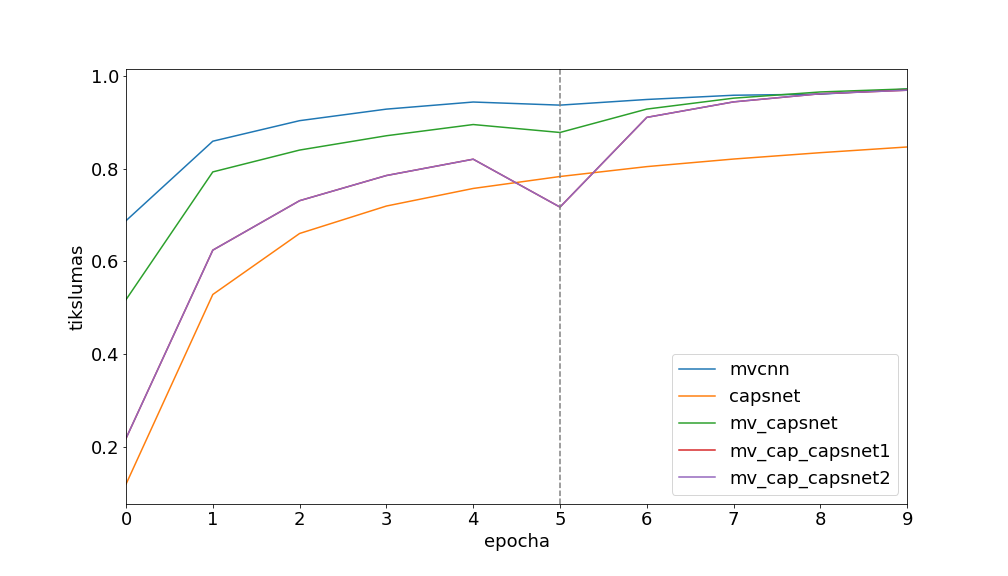
\includegraphics[scale=0.5]{img/trained.png}
	\caption{
		Apmokymo duomenų klasifikavimo tikslumas, kur mvcnn yra daugiavaizdžio neuroninio tinklo tikslumas, capsnet - kapsulinio neuroninio tinklo tikslumas, mv\_capsnet - daugiavaizdžio kapsulinio neuroninio tinklo su vaizdų sujungimo sluoksniu tikslumas, mv\_cap\_capsnet1 - daugiavaizdžio kapsulinio neuroninio tinklo su vaizdų kapsuliniu sluoksniu ir vienu mokymosi etapu tikslumas, mv\_cap\_capsnet2 - daugiavaizdžio kapsulinio neuroninio tinklo su vaizdų kapsuliniu sluoksniu ir dviem mokymosi etapais tikslumas. Brūkšninė vertikali linija nurodo antrojo apmokymo etapo pirmąją epochą.
	}
	\label{img:train_plot}
\end{figure}

\begin{figure}[H]
	\centering
	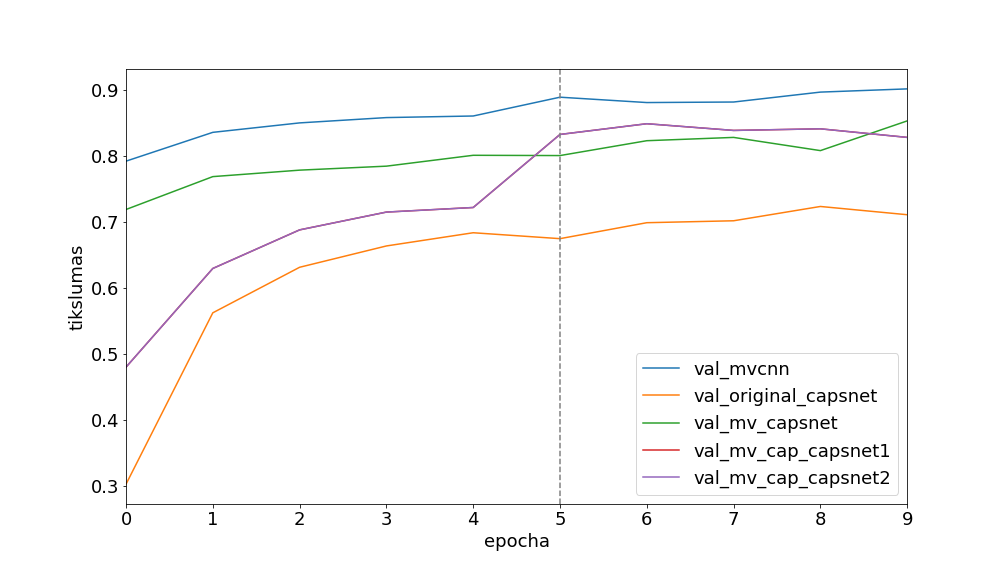
\includegraphics[scale=0.5]{img/validated.png}
	\caption{
		Testavimo duomenų klasifikavimo tikslumas, kur mvcnn yra daugiavaizdžio neuroninio tinklo tikslumas, capsnet - kapsulinio neuroninio tinklo tikslumas, mv\_capsnet - daugiavaizdžio kapsulinio neuroninio tinklo su vaizdų sujungimo sluoksniu tikslumas, mv\_cap\_capsnet1 - daugiavaizdžio kapsulinio neuroninio tinklo su vaizdų kapsuliniu sluoksniu ir vienu mokymosi etapu tikslumas, mv\_cap\_capsnet2 - daugiavaizdžio kapsulinio neuroninio tinklo su vaizdų kapsuliniu sluoksniu ir dviem mokymosi etapais tikslumas. Brūkšninė vertikali linija nurodo antrojo apmokymo etapo pirmąją epochą.
	}
	\label{img:val_plot}
\end{figure}
